\documentclass[a4paper,12pt]{article}

%%% Работа с русским языком
\usepackage{cmap}					% поиск в PDF
\usepackage{mathtext} 				% русские буквы в формулах
\usepackage[T2A]{fontenc}			% кодировка
\usepackage[utf8]{inputenc}			% кодировка исходного текста
\usepackage[english,russian]{babel}	% локализация и переносы

%%% Дополнительная работа с математикой
\usepackage{amsmath,amsfonts,amssymb,amsthm,mathtools} % AMS
\usepackage{icomma} % "Умная" запятая: $0,2$ --- число, $0, 2$ --- перечисление

%% Номера формул
%\mathtoolsset{showonlyrefs=true} % Показывать номера только у тех формул, на которые есть \eqref{} в тексте.
%\usepackage{leqno} % Нумерация формул слева

%% Свои команды
\DeclareMathOperator{\sgn}{\mathop{sgn}}

%% Перенос знаков в формулах (по Львовскому)
\newcommand*{\hm}[1]{#1\nobreak\discretionary{}
{\hbox{$\mathsurround=0pt #1$}}{}}

%%% Работа с картинками
\usepackage{graphicx}  % Для вставки рисунков
\graphicspath{{Materials/graphics/}{Materials/}}  % папки с картинками
\setlength\fboxsep{3pt} % Отступ рамки \fbox{} от рисунка
\setlength\fboxrule{1pt} % Толщина линий рамки \fbox{}
\usepackage{wrapfig} % Обтекание рисунков текстом

%%% Работа с таблицами
\usepackage{array,tabularx,tabulary,booktabs} % Дополнительная работа с таблицами
\usepackage{longtable}  % Длинные таблицы
\usepackage{multirow} % Слияние строк в таблице

%%% Теоремы
\theoremstyle{plain} % Это стиль по умолчанию, его можно не переопределять.
\newtheorem{theorem}{Теорема}[section]
\newtheorem{proposition}[theorem]{Утверждение}
 
\theoremstyle{definition} % "Определение"
\newtheorem{corollary}{Следствие}[theorem]
\newtheorem{problem}{Задача}[section]
 
\theoremstyle{remark} % "Примечание"
\newtheorem*{nonum}{Решение}

%%% Программирование
\usepackage{etoolbox} % логические операторы

%%% Страница
%\usepackage{extsizes} % Возможность сделать 14-й шрифт
\usepackage{geometry} % Простой способ задавать поля
	\geometry{top=25mm}
	\geometry{bottom=30mm}
	\geometry{left=25mm}
	\geometry{right=25mm}
 %

%%% Способ сделать тоже самое(но красивее:)
%\usepackage[margin=0.8in]{geometry}

 
\usepackage{fancyhdr} % Колонтитулы
 	\pagestyle{fancy}
 	\renewcommand{\headrulewidth}{0mm}  % Толщина линейки, отчеркивающей верхний колонтитул
 	\lfoot{}
 	\rfoot{}
 	\rhead{}
 	\chead{}
 	\lhead{ }
 	% \cfoot{Нижний в центре} % По умолчанию здесь номер страницы

\usepackage{setspace} % Интерлиньяж
%\onehalfspacing % Интерлиньяж 1.5
%\doublespacing % Интерлиньяж 2
%\singlespacing % Интерлиньяж 1

\usepackage{lastpage} % Узнать, сколько всего страниц в документе.

\usepackage{soulutf8} % Модификаторы начертания

\usepackage{hyperref}
\usepackage[usenames,dvipsnames,svgnames,table,rgb]{xcolor}
\hypersetup{				% Гиперссылки
    unicode=true,           % русские буквы в раздела PDF
    pdftitle={Заголовок},   % Заголовок
    pdfauthor={Автор},      % Автор
    pdfsubject={Тема},      % Тема
    pdfcreator={Создатель}, % Создатель
    pdfproducer={Производитель}, % Производитель
    pdfkeywords={keyword1} {key2} {key3}, % Ключевые слова
    colorlinks=true,       	% false: ссылки в рамках; true: цветные ссылки
    linkcolor=red,          % внутренние ссылки
    citecolor=green,        % на библиографию
    filecolor=magenta,      % на файлы
    urlcolor=cyan           % на URL
}

%\renewcommand{\familydefault}{\sfdefault} % Начертание шрифта

\usepackage{multicol} % Несколько колонок

% Мои "дополнительные" пакеты
\usepackage{textcase} 
\usepackage{pdfpages}
\usepackage{amsmath}
\usepackage{titlesec}
\usepackage{floatrow}



\author{Подкидышев Алексей}
\title{Студент МФТИ ФИВТ - 1ый курс}
\date{\today}

%% Делаем красивый header:
\fancyhead[RO]{\footnotesize{\scshape\nouppercase{~\leftmark}}}
%% Делаем красивый header END

%Делаем большой отступ между section и subsection
\titlespacing*{\section} {0pt}{3.5ex plus 1ex minus .2ex}{2.7ex plus .2ex}
\titlespacing*{\subsection} {0pt}{2.7ex plus 1ex minus .2ex}{1ex plus .2ex}


\begin{document} % конец преамбулы, начало документа


\begin{center}
	\textit{\MakeTextUppercase{федеральное государственное автономное учреждение}}
		
	\vspace{0.5ex}
	
	\textbf{ \\ \MakeTextUppercase{<<Московский Физико-технический институт>>}}
\end{center}
\vspace{13ex}
\begin{flushright}
	\noindent
	{Подкидышев Алексей Сергеевич}
	\\
	\textit{Студент факультета инноваций\\ и высоких технологий\\(группа 790)}
\end{flushright}
\begin{center}
	\vspace{23ex}
	\line(1,0){430}\\[4ex]
	{\LARGE\textbf{Лабораторная работа 2.1.1}}
	\vspace{2ex}
	
		
	\textbf{\large{<<Измерение удельной теплоемкости воздуха при постоянном давлении>>}}\\[3ex]
	\line(1,0){430}\\[5ex]
	\vfill
	Долгопрудный 
	
	{\today}
\end{center}

\newpage
\renewcommand{\headrulewidth}{1pt}

\section{Описание работы}
\subsection{Цель работы}\
\begin{enumerate}
\item Измерение повышения температуры воздуха в результате подвода    тепла   при   стационарном   течении   через   стеклянную  трубку.

\item
Вычисление по результатам измерений теплоемкости воздуха при постоянном давлении.
\end{enumerate}

\subsection{Оборудование}\
\indent Теплоизолированная трубка; электронагреватель; газовый счетчик; источник питания; термопара; вольтметр; амперметр; секундомер.

\subsection{Теория}

\subsection{Течение газа по трубе}
\begin{wrapfigure}{l}{0.75\textwidth} \label{pic:sheme}
	\includegraphics[width=0.8\linewidth]{pic2.jpg}
	\caption{Нагрев газа при течении по трубе}
\end{wrapfigure}
Теплоёмкость тела в некотором процессе определяется как их отношение:
\begin{equation}
C = \dfrac{\delta Q}{\vartriangle T}
\end{equation}\\[5ex]
\\
\\
В общем случае давление на входе может заметно превышать таковое на выходе (например, если труба доста-точно узкая и длинная). Рассмотрим течение газа более детально, чтобы выяснить пределы применимости соотношения \begin{large}
 $\frac{N - N_\text{пот}}{q\Delta T}$. 
\end{large}

Надёжность измерения определяется, в основном, качеством калориметра. Необходимо, чтобы количество тепла, затрачиваемое на нагревание исследуемого тела, существенно превосходило тепло, расходуемое на нагревание самого калориметра, а также на потери тепла из установки. При измерении теплоёмкости газов эти требования выполнить довольно трудно — масса газа в калориметре и, следовательно, количество тепла, идущее на его нагревание, как правило, малы. Для увеличения количества нагреваемого газа при неизменных размерах установки в нашей работе исследуемый газ (воздух) продувается через калориметр, внутри которого установлен нагреватель. При этом измеряются мощность нагревателя, масса воздуха, протекающего в единицу времени (расход), и приращение его температуры.(отмечено серым на рис. \ref{pic:sheme}) и применим к ней \textbf{закон сохранения энергии}.
Пусть за время d газ сместился слева направо на малое расстояние вдоль трубки, такое что через левую границу прошёл газ объёмом $dV_1$, а через правую $V_2$. В силу закона сохранения массы имеем:

\begin{equation}
dm = \rho_1 dV_1 = \rho_2 dV_2 
\end{equation}\

\indent В условии опыта измеряется именно \textit{удельная теплоемкость при постоянном давлении $C_p$}:

\begin{equation}
C_p = \dfrac{N - N_\text{пот}}{q \cdot \triangle T}
\end{equation}


\subsection{Схема установки}

\begin{wrapfigure}{l}{0.6\linewidth}\label{pic:sheme}

	\caption{Схема формирования потока газа в трубе круглово сечения}
	\includegraphics[width=\linewidth]{Scheme.png}
	
\end{wrapfigure}\
\\[5ex]
\indent Воздух, нагнетаемый компрессором, прокачивается через калориметр. Калориметр представляет собой стеклянную цилиндрическую трубку с двойными стенками, запаянными с торцов. Нагреватель в виде намотанной на пенопласт нихромовой проволоки рас-положен внутри калориметра непосредственно в воздушном потоке.

\begin{equation}
N = UI
\end{equation}
Для измерения разности температур $\triangle$ T служит медно-константановая термопара. Один спай термопары расположен в струе воздуха, входящего в калориметр, и находится при комнатной температуре, а второй в струе выходящего нагретого воздуха.

\begin{equation}
\varepsilon = \beta \cdot \Delta T
\end{equation}
где $\beta  = 40.7 \  \dfrac{\text{мкВ}}{C_\circ }$ чувствительность медно-константановой термопары в рабочем диапазоне температур (20–30 $C^\circ$)ЭДС регистрируется с помощью микровольтметра. Объём воздуха, прошедшего через калориметр, измеряется газовым счётчиком \textbf{ГС}. Для регулировки расхода служит кран \textbf{К}.

Объёмный расход равен $\Delta V/\Delta t$ , массовый расход может быть найден как
\begin{equation}
q = \rho_0 \dfrac{\Delta V}{\Delta t}
\end{equation}
где $\rho_0$ — плотность воздуха при комнатной температуре, которая в свою очередь может быть получена из уравнения Менделеева–Клапейрона:
\[ \rho_0 = \dfrac{\mu \cdot P_0}{R \cdot T_0}\]

\section{Ход работы}

\subsection{Подготовка}

\begin{itemize}
\item Измерим расход воздуха(объемный) при максимально открытом кране
\item Используя термометр, определим температуру и влажность воздуха. С помощью этих данных, определим значение $C_{\text{p}} \text{воздуха}$ 
\item Посчитаем мощность нагревателя, приняв значения сопротивления проволоки(которая используется в нагревателе) - 35 Ом
\end{itemize}

\begin{table}[H]
\centering
\caption{Оценка значения $ I_0 $ для $\Delta T = 1 \ C^\circ $ (Необходимо чтобы определить ток, с которого мы начнем делать измерения)}

\label{tab:tab1}
\begin{tabular}{|l|l|l|l|}
\hline
Q - расход воздуха, $kg/s$ & $C_p$ воздуха, $\dfrac{\text{Дж}}{kg * C^\circ} $ & N, Вт    & $I_0$, А     \\ \hline
9,52E-05               & 1119                                       & 0,107 & 0,055 \\ \hline
\end{tabular}
\end{table}

\begin{Large}
Итого:
\end{Large}

\begin{large}
\begin{center}
\begin{tabular}{|c|}
\hline 
$I_0 \approx 0,055$ A = 55 mA\\ 
\hline 
\end{tabular} 
\end{center}
\end{large}

\subsection{Измерения(1-ая серия)}
\subsubsection{Таблица}
\indent Измереним $\triangle T (U_{источкника})$ при максимальном расхдоде
\textbf{\large{Q = 0.074 $\dfrac{l}{s}$}}:

\begin{table}[h]
\centering
\caption{Таблица измерений $\Delta T$ - разности температур воздуха на разных участках(Холодного и теплового воздуха, N - мощности нагревателя. \textit{При максимальном расходе воздуха}}
\label{tab:tab1}
\begin{tabular}{|l|l|l|l|l|}
\hline
I, mA & U, В  & Напряжение на термопаре, mV & $\Delta T, C^\circ$ & N, 10\textasciicircum -3 \\ \hline
51,5  & 1,477 & 0,01                        & 0,246               & 91,50263                 \\
79    & 2,2   & 0,032                       & 0,786               & 215,3145                 \\
104,2 & 2,9   & 0,083                       & 2,039               & 374,5886                 \\
135,9 & 3,9   & 0,138                       & 3,391               & 637,1739                 \\
160,2 & 4,601 & 0,2                         & 4,914               & 885,4094                 \\
211,9 & 6,083 & 0,367                       & 9,017               & 1549,106                 \\ \hline
\end{tabular}
\end{table}

\begin{figure}[H]
{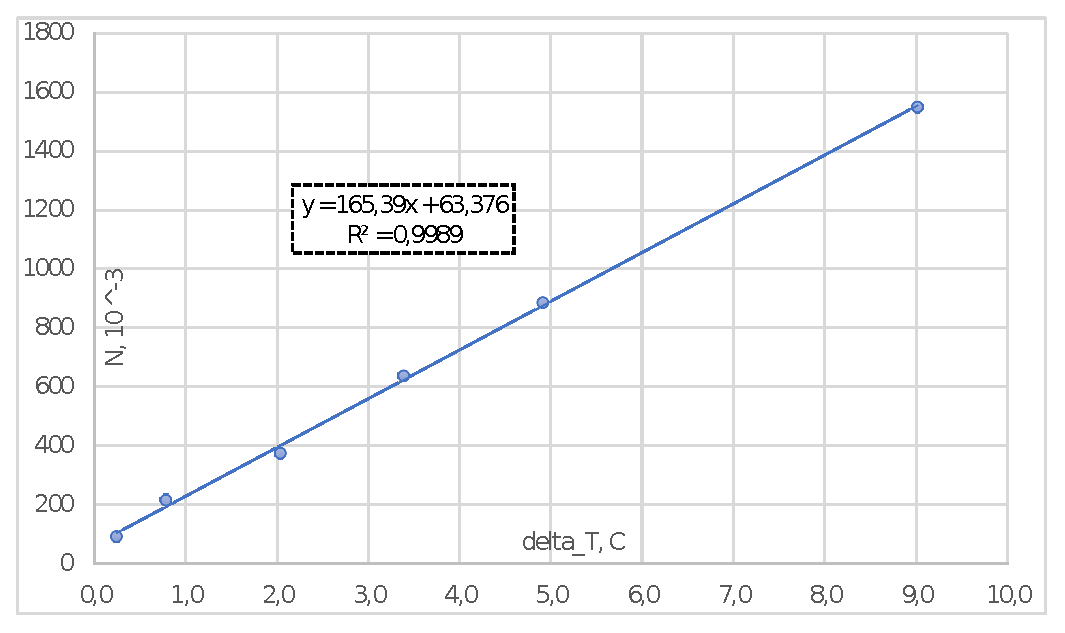
\includegraphics[width=1\linewidth]{graph1.eps}}
\caption{График зависимости N($\Delta T$) - Мощности нагревателя(Разности температур), коэффициент наклона прямой, необходим для расчета $C_p$. \textit{При максимальном расход воздуха}}
\end{figure}

\subsubsection{Измерение угла наклона}
Для того чтобы посчитать $C_p$ необходимо знать график угла наклона графика. В 
том случае погрешность измеряется по формуле:

\begin{equation}
k = \dfrac{<xy> - <x> \cdot <y>}{<x^2> - <x>^2}
\end{equation}

\begin{equation}
\sigma_k = \dfrac{1}{\sqrt{n}} \sqrt{\dfrac{<y^2> - <y>^2}{<x^2> - <x>^2} - k^2}
\end{equation}

\large{Итогове значение для k}:
\[k = \frac{P}{\Delta T} = 0.165 \pm 0.005 \]

\subsubsection{Результат}
По измеренным данным определим значение $C_p$, по формуле:
\[C_p = \dfrac{P}{\Delta T \cdot q} - \dfrac{\alpha}{q} \]

\begin{center}
\begin{tabular}{|c|}
\hline 
$C_p = 1732 \pm 70 \dfrac{\text{Дж}}{kg * C^\circ} $ \\ 
\hline 
\end{tabular} 
\end{center}

\subsection{Измерения. 2-ая серия}\
Измерим $\triangle T (U_{источкника})$ при \textbf{\large{Q =  0,0385 $\dfrac{l}{s}$}}:

\begin{table}[h]
\centering
\caption{Таблица измерений $\Delta T$ - разности температур воздуха на разных участках(Холодного и теплового воздуха, N - мощности нагревателя. \textit{При  расходе воздуха = 0,0385 $\dfrac{l}{s}$}}
\label{tab:tab2}
\begin{tabular}{|l|l|l|l|l|}
\hline
I, mA & U, В  & Напряжение на термопаре, mV & $\Delta T, C^\circ$ & N, $10^{ -3}$, Вт \\ \hline
91,3  & 2,621 & 0,09                        & 2,211               & 287,5813                 \\
134,5 & 3,861 & 0,203                       & 4,988               & 624,1136                 \\
162,3 & 4,662 & 0,316                       & 7,764               & 908,7745                 \\
207,3 & 5,953 & 0,531                       & 13,047              & 1482,579                 \\ \hline
\end{tabular}
\end{table}

\begin{figure}[H]
{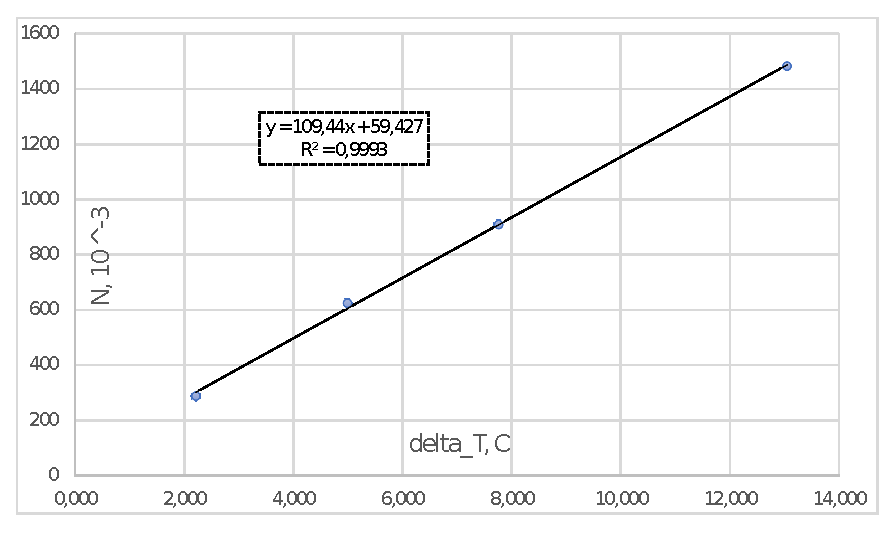
\includegraphics[width=1\linewidth]{graph2.eps}}
\caption{График зависимости N($\Delta T$) - Мощности нагревателя(Разности температур), коэффициент наклона прямой, необходим для расчета $C_p$.
\mbox{При  расходе воздуха = 0,0385 $\dfrac{l}{s}$}}
\end{figure}

\indent Аналогично первой серии измерений посчитаем погрешности и значение $C_p$(пользуясь формулами \textbf{7,8}):\\[1ex]

\begin{center}
\begin{tabular}{|c|}
\hline 
$C_p = 1145 \pm 60 \dfrac{\text{Дж}}{kg * C^\circ} $ \\ 
\hline 
\end{tabular} 
\end{center}

\numberwithin{equation}{section}

\subsection{Доля теплопотерь в установке}\
\indent Мы получили $C_\text{ фактическая} = 1400 \pm 200\  \dfrac{\text{Дж}}{kg \cdot C^\circ} $ (что отличается от табличного значения - 1119 $  \frac{\text{Дж}}{\text{кг} \cdot C^\circ}$)

\begin{equation*}
N = \alpha * \Delta T = C_{p\text{ фактическая}} * \Delta T\  - \ C_{p\text{ теоритическая}} * \Delta T
\end{equation*}

\begin{equation*}
\alpha = C_{p\text{ фактическая}}\  -\  C_{p\text{ теоритическая}} 
\end{equation*}

\begin{equation*}
\frac{P}{N} = \frac{C_{p\text{ теоритическая}} + \alpha}{\alpha} =  \frac{ C_{p\text{ фактическая}}}{ C_{p\text{ фактическая}} -  C_{p\text{ теоритическая}}} \simeq 2.9
\end{equation*}

\section{Вывод}
\begin{itemize}
\item Теоретическая теплоемкость воздуха и его экспериментальная теплоемкость, искаженная тепловыми потерями \textbf{отличаются примерно на $2\sigma$}, что говорит о больших тепловых потерях, не учтенных в погрешности. В пользу этого говорит возрастание ошибки определения теплоемкости при уменьшении скорости потока, воздух проводит в термостате больше времени, теряет больше тепла

\item Оценка средней доли теплопотерь подтвердила предположения: в среднем воздух теряет около \textbf{трети} полученного от нагревателя тепла через стенки термостата.
\end{itemize}

\end{document}